\apendice{Documentación técnica de programación}

\section{Introducción}
Esta sección está dirigida a otros desarrolladores, de modo que puedan continuar el proyecto y entenderlo. En él se describen en detalle el funcionamiento del proyecto y los aspectos que podrían mejorarse o modificarse en el futuro.
\section{Estructura de directorios}

\subsection{Ejecutables:} 
	\begin{itemize}
		\item EjecutarGui: Este fichero se corresponde con el ejecutable para lanzar la aplicación en modo GUI.
		\item EjecutarTest: Este fichero se corresponde con el ejecutable para lanzar los test de la aplicación en modo consola.
		\item Documentar: Este fichero se corresponde con el ejecutable para documentar la aplicación de forma recursiva y crear los ficheros HTML correspondientes.
	\end{itemize}
		
\subsection{Documentación:}
En esta carpeta está contenida la documentación en formato HTML.
	\begin{itemize}
		\item pydoc: Esta carpeta se corresponde con la documentación de pydoc
	\end{itemize}

\subsection{Src:}
Esta carpeta contiene todos los ficheros de código fuente del proyecto, el OCR, y los test.

\subsubsection{Proyecto:}
Esta carpeta corresponde todos los ficheros de código fuente del proyecto, todos los módulos o paquetes.

\textbf{Análisis}
\begin{itemize}
	\item Estadísticas.
		\begin{itemize}
			\item Estadística.
		\end{itemize}
	\item Informes:
		\begin{itemize}
			\item ConfiguracionToXML.
			\item DatosToCsv.
			\item Informe.
			\item InGuardarDatos
		\end{itemize}
	\item Procesado:
		\begin{itemize}
			\item ProcesadoAutomatico.
			\item ProcesadoDeImagen
			\item ProcesadoDeLineas
		\end{itemize}
	\item Diccionario:
		\begin{itemize}
			\item Diccionario
			\item DiccionarioING
		\end{itemize}
	\item FachadaBotonesAndLayaout.
	\item FachadaEntradaSalida.	
	\item MediadorPestannas.
	\item MediadorVentana.
\end{itemize}	

\textbf{GUI}
\begin{itemize}
		\item PanelDePestannas
		\item PintarRectangulo
		\item VentanaInicio
		\item VisorHtml
		\item Window
\end{itemize}

\subsubsection{Tesseract:}
Esta carpeta contiene el ejecutable del OCR junto con sus ficheros de configuración para poderlo ejecutar.

\subsection{Test:}
Esta carpeta contiene los test del código para comprobar que funcionan correctamente.
\subsubsection{Codigo:}
\begin{itemize}
	\item Estadísticas:
		\begin{itemize}
			\item TestEstadistica
		\end{itemize}
	\item Informes:
		\begin{itemize}
			\item TestConfiguracionToXML
			\item TestDatosToCsv
			\item TestInforme
		\end{itemize}
	\item Procesado:
		\begin{itemize}
			\item TestProcesadoDeImagen
			\item TestProcesadoDeLineas
		\end{itemize}
\end{itemize}

\section{Manual del programador}
En esta sección vamos a describir como se han programado las partes mas importantes que son las que mas nos interesan.
\subsection{Procesado}
Para programar el procesado hemos encadenado sucesivos pasos, que dividiremos en tres secciones.

\begin{itemize}
\item ProcesadoDeImagen: Este se corresponde con el procesado de la imagen para la extracción de las características.
	\begin{enumerate}

	\item Hemos calculado de la imagen la distancia a un color: Se corresponde con el que estén pintadas los segmentos, lo selecciona el usuario. Evitamos cualquier color que hiciese que falle el algoritmo, filtrando la selección por el canal del modelo de color HSV, que indica la saturación. En nuestra imagen lo único que tiene una saturación alta son los segmentos pintados ya que la imagen esta en escala de grises.

	\item Binarizamos la imagen con la distancia al color para obtener la máscara con los objetos que queremos detectar y reducimos el grosor de estos.

	\item Sobre la máscara reducida calculamos los segmentos por la transformada de Hough.
	\end{enumerate}

\item ProcesadoDeLineas: Este módulo contiene el procesado de las lineas, detectadas en el último paso del punto anterior.
\begin{enumerate}

\item Primero de todo, lo que tenemos no son segmentos completos, sino subsegmentos que forman los segmentos reales. Tenemos que unirlos aquellos que sean muy similares, caracterizados por distancia y ángulo.

\item Para realizar la unión lo primero que haremos será ir añadiendo, un camino entre los dos segmentos, a un grafo, de aquellos que cumplan lo anterior.

\item Obtendremos las uno componentes del grafo \footnote{Se explica en las memorias pero podemos encontrarlo aquí también \cite{Wiki:Grafos}}, que se corresponden, con los clusters, que son los segmentos buscados.
\end{enumerate}

\item ProcesadoAutomatico: Este apartado aunque lleva proceso similares a los anteriores no puede ir junto ya que necesita otros pasos intermedios.
\begin{enumerate}

\item Usaremos el detector de bordes que hemos implementado.
\item Ecualizaremos la imagen para distribuir su histograma.
\item Calculamos los autovectores de la matriz Hessiana y nos quedamos con los autovectores largos.
\item Binarizamos la imagen y procesamos dicha imagen. Queda reflejado en anexo \ref{anexo:F}.
\end{enumerate}

\end{itemize}

\subsection{GUI}

\begin{itemize}
	\item Imagen y líneas: Para pintar las imágenes, hemos usado el backend de Matplotlib, que nos muestra la imagen sobre unos ejes de coordenadas, que nos indican e informan sobre las coordenadas de cada pixel. Gracias a esto y a los métodos de conexión sobre los eventos, hemos podido simplificar al máximo la obtención de los puntos, la forma de pintar los segmentos detectados y la interacción de usuario.
	
	\item OCR: Para leer la referencia de la imagen hemos usado un OCR conocido que se llama Tesseract. Le pasamos el recorte de la imagen que contiene la referencia y nos devuelve el numero que contiene.
\end{itemize}

\section{Compilación, instalación y ejecución del proyecto}

\subsection{Compilación:}
En Python no hace falta compilar el proyecto ya que es un lenguaje interpretado. Necesitaremos únicamente tener Python instalado, a través de Miniconda o cualquier otra distribución, de Python.

Python es un lenguaje interpretado y necesitamos tener Python 3.5. junto con las librerías usadas, pero instalar una a una dichas librerías es un trabajo complejo, para un usuario. Por eso para facilitar la instalación de Python hemos optado por usar Miniconda, es una distribución que facilita dicha instalación pero sin ninguna librería instalada, por lo que es mas ligero, 50 Megas, frente a Anaconda, cerca de 500 Megas. Quedando a nuestra disposición indicar que librerías instalar.

En la primera ejecución del código nos va a descargar e instalar todas las librerías que necesitamos.

\subsection{Instalación:}
Para poder ejecutar deberemos instalar Miniconda en 
 \textrm{C\textbackslash Users\textbackslash TuUsuario}, Es el directorio predefinido por Miniconda, una vez que lo tengamos instalado podremos proceder a hacer doble clic sobre el ejecutable  \textrm{EjecutarGui.bat} que instalará las dependencias a las librerías que necesitamos para su ejecución.

\subsection{Ejecución del proyecto:}
Para la primera ejecución, si no tenemos las librerías instaladas, al hacer doble clic sobre EjecucionGui.bat, tardará un rato en descargarlas y crear el entorno virtual de Miniconda con únicamente las librerías que se usan. No obstante, en lo sucesivo únicamente ejecutara la aplicación.

Si la descarga de las librerías se interrumpe por una caída de la red u otro problema, nos dará un error. Pero si volvemos a ejecutar, se iniciará donde se paró la descarga, es decir no perdemos lo que ya haya conseguido descargar.


\subsection{Conclusiones:}
Hemos seguido otras formas de conseguir crear un entorno de ejecución, hemos intentado crear el ejecutable como se detalla en las memorias pero no hemos sido capaces, por problemas de versiones, aun no están disponibles.



\section{Pruebas del sistema}
En esta sección vamos a informar como ejecutar los test que están ubicados en la carpeta Test dentro de la carpeta src del proyecto. 

\subsection{Test Python:}
Dichos test están escritos en Python usando la librería unittest.

Hay muchas comprobaciones sobre las funciones de cálculo y aquellas que escriben y leen ficheros, pero para la parte de la interfaz gráfica no hay hechas pruebas ya que no se puede controlar del todo esta part. Pero ha sido probada por mí y todos los aspectos añadidos y no produce fallos conocidos.

Para ejecutarlos basta con ejecutarlos desde Eclipse, el main de los test mainTest.py o también si preferimos podemos ejecutarlos desde la terminal con el mismo fichero.
Otra opción para ejecutar los test es dar doble clic sobre el ejecutable EjecutarTest que esta en la carpeta de los ejecutables. 

Aparte de los datos proporcionados en la ejecución hemos puesto una salida informativa para cada test y las partes que comprueba.
 
\subsection{Test de calidad}
En este apartado vamos a mostrar las medidas que vamos a usar para conseguir la calidad de las imágenes y explicar las formulas obtenidas de \cite{wiki:confMatrix}.

Para una mejor clasificación y obtener unas medidas tangibles hemos optado por usar la clásica matriz de confusión que diferencia 4 valores como podemos observar en la tabla \ref{tab:ConfMatrix}.

\begin{itemize}
\item True positive rate (TPR): Mide la proporción de los elementos que se han considerado como positivos y son positivos.
\[TPR=\frac{TP}{TP+FN}\]

\item True negative rate (TNR):Mide la proporción de los elementos que se han considerado como negativos y son negativos. 
\[TNR=\frac{TN}{FP+TN}\]

\item Positive predictive value (PPV): Mide la proporción de elementos clasificados como verdaderos positivos entre los positivos.
\[PPV=\frac{TP}{TP+FP}\]


\item Negative predictive value (NPV): Mide la proporción de elementos clasificados como verdaderos negativos entre los negativos.  
\[NPV=\frac{TN}{TN+FN}\]


\item False positive rate (FPR):
Mide la proporción de los elementos que se han considerado como falsos positivos entre los que son negativos reales.
 \[FPR=1-TNR\]

\item False discovery rate (FDR):
Mide la proporción de los elementos que se han considerado como falsos positivos entre los que son positivos de verdad.
\[FDR=1-PPV\]

\item Miss rate or false negative rate (FNR):
Mide la proporción de los elementos que se han considerado como falsos negativos entre los que son  positivos. \[FNR=1-TPR\]

\item Accuracy (ACC): Mide el error observable.
\[ACC=\frac{TP+TN}{P+N}\]

\item Valor F1: Este valor muestra la media armónica entre la precision y la sensibilidad del modelo.
\[F1=\frac{2TP}{2TP+FP+FN}\]

\item Matthews correlation coefficient (MCC):
Esta medida se usa en Maching Learning para medir la calidad de la clasificación en dos clases \cite{wiki:machineMCC}.
 \[MCC=\frac{TP*TN-FP*FN}{\sqrt{(TP+FP)*(TP+FN)*(TN+FP)*(TN+FN)}}\]
 
\item Informedness or Bookmaker Informedness (BM):
Esta medida informa de la generalización de un problema multi-clases y estima la probabilidad de decisión.
 \[BM=TPR+TNR-1\]

\item Markedness (MK):
Esta es la medida de cuando una variable es marcada como predicción o causa posible de otra.
 \[MK=PPV+NPV-1\]


\end{itemize}



\subsubsection{Pruebas}
Aquí van a aparecer una muestra de las pruebas que hemos realizado sobre la aplicación para medir la calidad de la detección.


Para las pruebas vamos a optar por construir una matriz de confusion sobre los resultados, la tabla mostrada a continuación, sera el modelo que vamos a seguir \ref{tab:ConfMatrix}.

\begin{table}
  \begin{center}
    \begin{tabular}{c l c c}
                 &                & \multicolumn{2}{c}{\cellcolor{brown!25}Predicted condition}   \\
                 &                & \cellcolor{brown!15}Positive prediction & \cellcolor{brown!45}Negative prediction \\
       \cellcolor{blue!15}True      & \cellcolor{blue!10}Positive class & \cellcolor{green!25}True positive (TP)  & \cellcolor{red!25}False negative (FN) \\
       \cellcolor{blue!15}Condition & \cellcolor{blue!30}Negative class & \cellcolor{red!25}False positive (FP) & \cellcolor{green!25}True negative (TN)  \\
    \end{tabular}
  \end{center}
  \caption{Estructura de la matriz de confusion.}
  \label{tab:ConfMatrix}
\end{table}



Prueba 1: La matriz de confusión obtenida para esta prueba la podemos observar en la tabla \ref{tab:pruebas}.
Las imágenes original, como muestra la figura \ref{fig:orip1}, y calculada, como muestra la figura \ref{fig:calcp1}, las podemos observar en la figura \ref{fig:p1}.
Los resultados de las medidas de calidad se muestran en la tabla \ref{tab:parte}.

Prueba 2: La matriz de confusión obtenida para esta prueba la podemos observar en la tabla \ref{tab:pruebas}.
Las imágenes original, como muestra la figura \ref{fig:orip2}, y calculada, como muestra la figura \ref{fig:calcp2}, las podemos observar en la figura \ref{fig:p2}.
Los resultados de las medidas de calidad se muestran en la tabla \ref{tab:parte}.

Prueba 3: La matriz de confusión obtenida para esta prueba la podemos observar en la tabla \ref{tab:pruebas}.
Las imágenes original, como muestra la figura \ref{fig:orip3}, y calculada, como muestra la figura \ref{fig:calcp3}, las podemos observar en la figura \ref{fig:p3}.
Los resultados de las medidas de calidad se muestran en la tabla \ref{tab:parte}.

Prueba 4: La matriz de confusión obtenida para esta prueba la podemos observar en la tabla \ref{tab:pruebas}.
Las imágenes original, como muestra la figura \ref{fig:orip4}, y calculada, como muestra la figura \ref{fig:calcp4}, las podemos observar en la figura \ref{fig:p4}.
Los resultados de las medidas de calidad se muestran en la tabla \ref{tab:parte}.




\begin{table}[]
\centering
\caption{Tabla de resultados matriz de confusión}
\label{tab:pruebas}
\begin{tabular}{@{} lrrrr @{}}
\hline
Prueba                & True positive & False negative & False positive & True negative \\ \hline
Figura \ref{fig:p1} & 36136         & 3840           & 3685           & 1185139       \\ \hline
Figura \ref{fig:p2} & 31670         & 844            & 6514           & 1189772       \\ \hline
Figura \ref{fig:p3} & 23114         & 8238           & 7103           & 1190345       \\ \hline
Figura \ref{fig:p4} & 30284         & 1773           & 14753          & 1181990       \\ \hline
\end{tabular}
\end{table}



\begin{table}[]
\centering
\caption{Resultados medidas de calidad}
\label{tab:parte}
\resizebox{\textwidth}{!}{
\begin{tabular}{@{} lllllllllllllll @{}}
\hline
Prueba                & TPR  & TNR  & PPV  & NPV  & FPR   & FDR  & FNR  & ACC  & F1   & MCC  & BM   & MK   \\ \hline
Figura \ref{fig:p1} & 0.90 & 0.99 & 0.99 & 0.99 & 0.003 & 0.09 & 0.09 & 0.99 & 0.91 & 0.90 & 0.9  & 0.90 \\ \hline
Figura \ref{fig:p2} & 0.97 & 0.99 & 0.83 & 0.99 & 0.17  & 0.17 & 0.02 & 0.99 & 0.90 & 0.90 & 0.83 & 0.82 \\ \hline
Figura \ref{fig:p3} & 0.74 & 0.99 & 0.76 & 0.99 & 0.01  & 0.24 & 0.26 & 0.99 & 0.75 & 0.74 & 0.73 & 0.76 \\ \hline
Figura \ref{fig:p4} & 0.94 & 0.99 & 0.67 & 0.99 & 0.01  & 0.33 & 0.05 & 0.99 & 0.78 & 0.79 & 0.93 & 0.67 \\ \hline
Media & 0.88 & 0.99 & 0.81 & 0.99 & 0.04  & 0.20 & 0.11 & 0.99 & 0.84 & 0.83 & 0.85 & 0.78 \\ \hline
Desviación & 0.10 & 0 & 0.13 & 0 & 0.08  & 0.10 & 0.10 & 0 & 0.08 & 0.08 & 0.08 & 0.09 \\ \hline
\end{tabular}
}
\end{table}



\begin{figure}
	\begin{subfigure}[c]{.5\linewidth}
	\centering\large 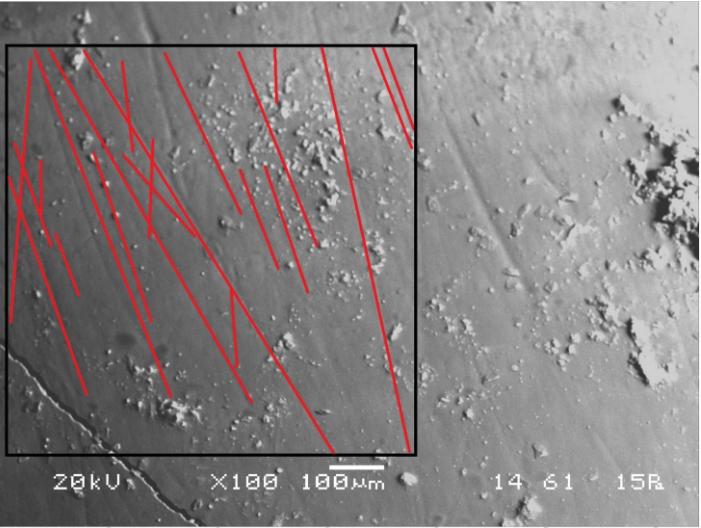
\includegraphics[width=.9\textwidth]{prueba1Ori}
	\caption{Estrías pintadas por el usuario prueba 1.}\label{fig:orip1}
	\end{subfigure}%
	\begin{subfigure}[c]{.5\linewidth}
	\centering\large 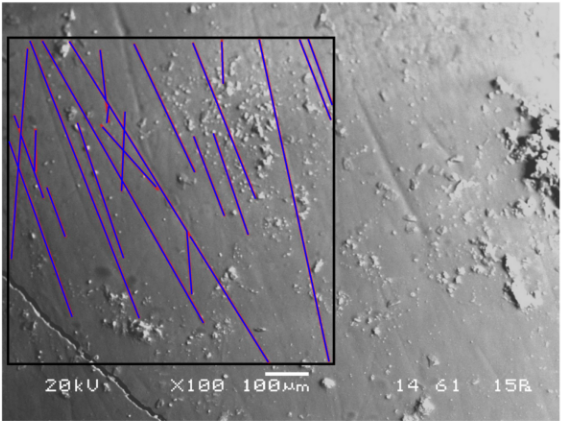
\includegraphics[width=.9\textwidth]{prueba1Detec}
	\caption{Estrías pintadas por la aplicacion prueba 1.}\label{fig:calcp1}
	\end{subfigure}%
	\caption{Imágenes prueba 1}
	\label{fig:p1}
\end{figure}



\begin{figure}
	\begin{subfigure}[c]{.5\linewidth}
	\centering\large 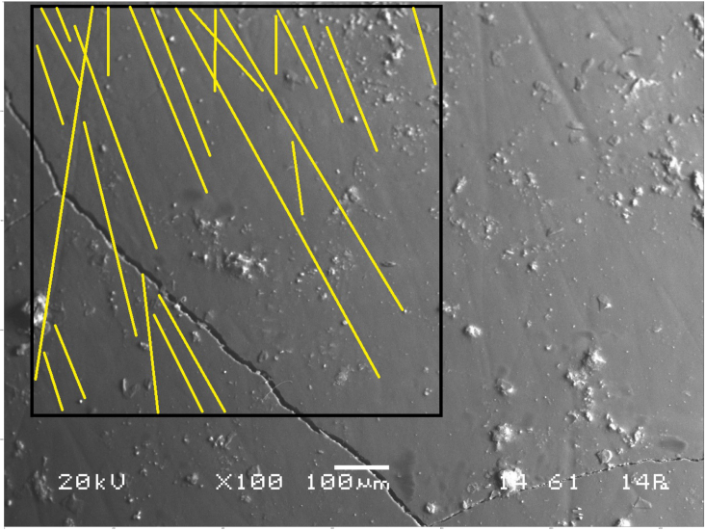
\includegraphics[width=.99\textwidth]{prueba2Ori}
	\caption{Estrías pintadas por el usuario prueba 2.}\label{fig:orip2}
	\end{subfigure}%
	\begin{subfigure}[c]{.5\linewidth}
	\centering\large 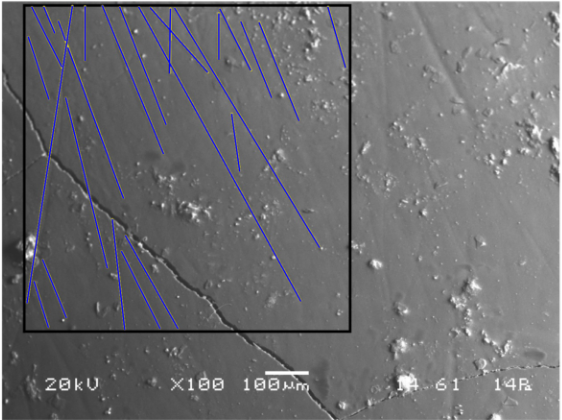
\includegraphics[width=.99\textwidth]{prueba2Detec}
	\caption{Estrías pintadas por la aplicacion prueba 2.}\label{fig:calcp2}
	\end{subfigure}%
	\caption{Imágenes prueba 2}
	\label{fig:p2}

\end{figure}


\begin{figure}
	\begin{subfigure}[c]{.5\linewidth}
	\centering\large 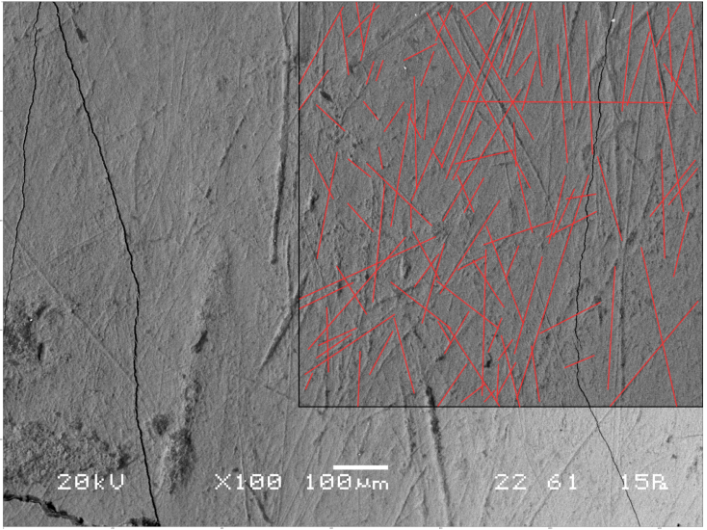
\includegraphics[width=.9\textwidth]{prueba3Ori}
	\caption{Estrías pintadas por el usuario prueba 3.}\label{fig:orip3}
	\end{subfigure}%
	\begin{subfigure}[c]{.5\linewidth}
	\centering\large 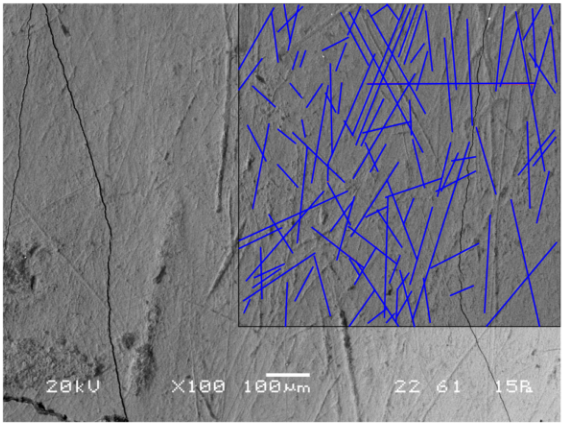
\includegraphics[width=.9\textwidth]{prueba3Detec}
	\caption{Estrías pintadas por la aplicacion prueba 3.}\label{fig:calcp3}
	\end{subfigure}%
	\caption{Imágenes prueba 3}
	\label{fig:p3}

\end{figure}



\begin{figure}
	\begin{subfigure}[c]{.5\linewidth}
	\centering\large 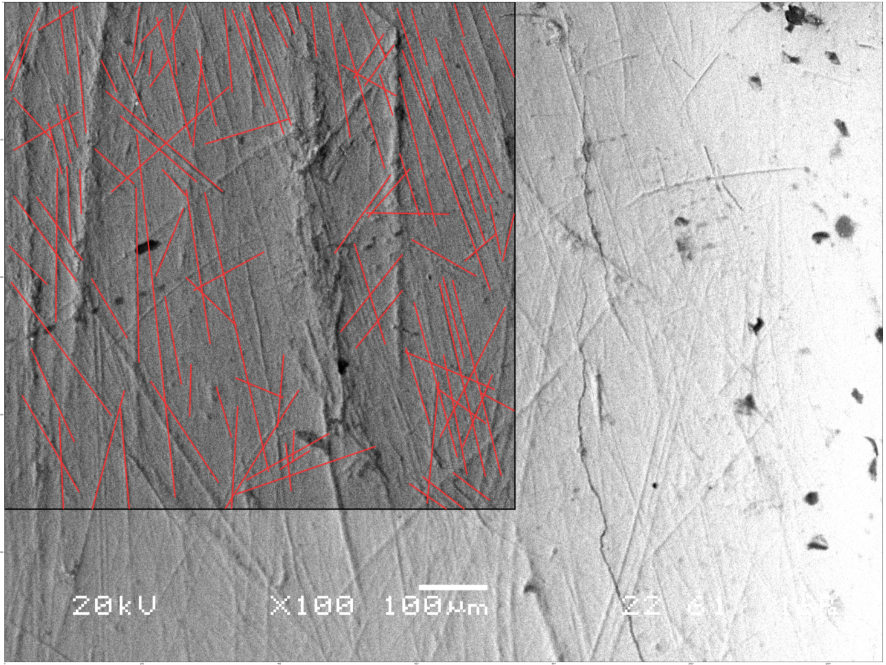
\includegraphics[width=.9\textwidth]{prueba4Ori}
	\caption{Estrías pintadas por el usuario prueba 4.}\label{fig:orip4} 
	\end{subfigure}%
	\begin{subfigure}[c]{.5\linewidth}
	\centering\large 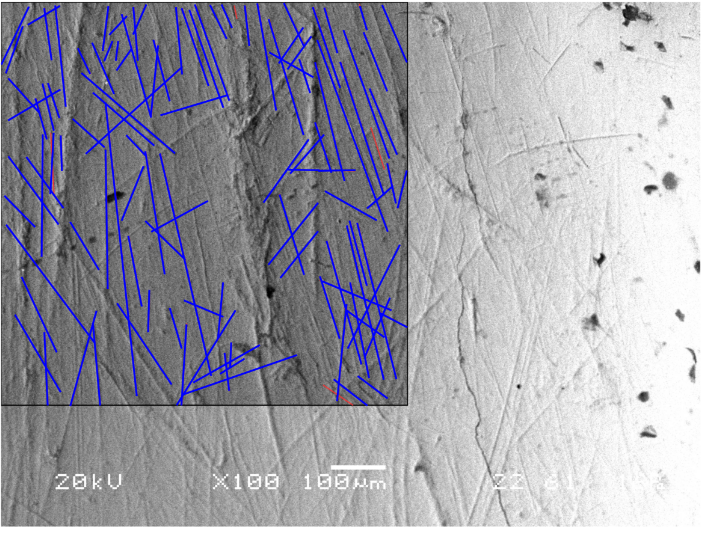
\includegraphics[width=.9\textwidth]{prueba4Detec}
	\caption{Estrías pintadas por la aplicacion prueba 4.}\label{fig:calcp4}
	\end{subfigure}%
	\caption{Imágenes prueba 4}
	\label{fig:p4}

\end{figure}
